\documentclass[12pt,a4paper,parskip=full]{scrartcl}

\usepackage{bbding}
\usepackage{pifont}
\usepackage{wasysym}
\usepackage[margin=1in]{geometry}
\geometry{letterpaper}
\usepackage{xcolor}
\definecolor{red}{HTML}{cc0000}
\definecolor{gray}{HTML}{666666}
\usepackage{sectsty}
\sectionfont{\color{red}}
\subsectionfont{\color{red}}
\usepackage{graphicx}
\usepackage{hyperref}
\usepackage{amssymb}
\usepackage[style=footnote-dw]{biblatex}
\bibliography{S@SGuideBib}
\setlength\bibitemsep{0.5\baselineskip}

\usepackage{enumitem}
\setitemize{noitemsep}
% \setlist{noitemsep, topsep=-5pt}
% \setlength\itemsep{-0.10em}

\renewcommand{\labelitemi}{$\cdot$}
\renewcommand{\labelitemii}{$\cdot$}
\makeatletter
\let\latexl@section\l@section
\def\l@section#1#2{\begingroup\let\numberline\@gobble\latexl@section{#1}{#2}\endgroup}
\makeatother

\usepackage[T1]{fontenc}
\fontfamily{verdana}

\usepackage{scrlayer-scrpage}{}
\makeatletter
\renewcommand{\@seccntformat}[1]{}
\makeatother

\setlength\parindent{0pt}{}

\title{\Huge{\color{red}\textbf{La Guida a Scrum@Scale
\textsuperscript{\copyright}
}}}
\subtitle{\color{gray}La guida definitiva a Scrum@Scale:\\ Lo scaling che funziona}
% \author{}
\date{}


\begin{document}

%\tableofcontents
%\newpage

\section{Scopo della Guida a Scrum@Scale}
Scrum, come originariamente descritto nella Scrum Guide, è un 
framework per sviluppare, consegnare e mantenere prodotti complessi da 
un singolo team. Fin dalla nascita, il suo uso si è esteso alla creazione di 
prodotti, processi, servizi e sistemi che richiedevano il lavoro di più team.
Scrum@Scale è stato creato per coordinare efficientemente questo nuovo 
ecosistema di team in un modo da ottimizzarsi per perseguire la strategia 
globale dell'organizzazione. Viene raggiunto questo obiettivo creando la 
minima burocrazia possibile grazie ad una architettura scale-free (architettura ad invarianza di scala - ndt), che estende naturalmente il modo in cui i singoli team Scrum funzionano lungo tutta l'organizzazione.

Questa guida contiene la definizione dei componenti che costituiscono Scrum@Scale, includendo i corrispondenti su larga scala dei ruoli, degli eventi, degli artefatti di Scrum e le regole che li tengono insieme.

Il Dr. Jeff Sutherland ha sviluppato Scrum@Scale basandosi sui principi fondamentali di Scrum, sulla teoria dei sistemi adattivi complessi, sulla teoria dei giochi e sulla programmazione ad oggetti. Questa guida è stata sviluppata grazie ai suggerimenti di numerosi esperti praticanti di Scrum ed è basata sui risultati del loro lavoro. L'obiettivo di questa guida è di rendere il lettore in grado di implementare Scrum@Scale in autonomia.

\subsection{Perché Scrum@Scale?}
Scrum è stato disegnato per permettere ad un singolo team di lavorare 
alla sua capacità ottimale mantenendo un ritmo sostenibile. Sul campo è
stato notato che all'aumentare dei team Scrum all'interno di una organizzazione,
la produzione (di prodotto funzionante) e la velocity di questi team iniziava a
decadere (a causa di problemi come le dipendenze tra team e la duplicazione
del lavoro). Diventava quindi ovvio che serviva un framework per coordinare 
efficacemente questi team in modo da ottenere una scalabilità lineare.
Scrum@Scale è stato ideato per raggiungere questo obiettivo grazie alla
sua architettura scale-free.

Utilizzando un'architettura scale-free, l'organizzazione non è 
vincolata a crescere in un particolare modo o secondo un insieme arbitrario di
regole; invece può crescere in maniera organica basandosi sui suoi personali
bisogni e ad un ritmo di cambiamento sostenibile, che possa essere 
accettato dai gruppi e dagli individui che compongono l'organizzazione.

Scrum@Scale è pensato per estendersi lungo tutta l'organizzazione: tutti
i dipartimenti, prodotti e servizi. Può essere applicato in diversi domini
e su qualsiasi tipo di organizzazione sia nell'industria, nei governi o nelle accademie.

\subsection{Definizione di Scrum@Scale}
Scrum: Un framework con cui le persone possono risolvere problemi adattivi complessi,
realizzando creativamente prodotti funzionanti con il più alto valore possibile.

La Scrum Guide è l'insieme minimo di regole che permettono ispezione e adattabilità
attraverso una trasparenza radicale per creare innovazione, soddisfazione dei clienti,
performance e felicità del team.

Scrum@Scale: Un framework con cui una rete di team Scrum opera in maniera consistente
alla Scrum Guide per indirizzare problemi adattivi complessi producendo e creando creativamente dei prodotti funzionanti del più alto valore possibile.

\textbf{NOTA:} Questi ``prodotti'' possono essere hardware, software, sistemi complessi integrati, processi, servizi, ecc., a seconda del dominio dei team Scrum.

Scrum@Scale è:
\begin{itemize}
\item Leggero - la minima burocrazia sostenibile
\item Semplice da capire - consiste soltanto di team Scrum
\item Difficile da padroneggiare - richiede di implementare un nuovo modello operativo
\end{itemize}

Scrum@Scale è un framework per scalare Scrum (estendere Scrum ad una scala più ampia - ndt). Questo è semplificato radicalmente in quanto si usa Scrum per scalare Scrum.

In Scrum, è stato separata con cura la responsabilità del ``cosa'' dal ``come''.
La stessa cura è stata mantenuta in Scrum@Scale in modo che la giurisdizione e le responsabilità siano espressamente comprese in modo da eliminare conflitti organizzativi e sprechi che impediscano ai team di raggiungere la loro produttività ottimale.

Scrum@Scale è costituito da componenti che consentono ad un'organizzazione di personalizzare la propria strategia di trasformazione e implementazione. Permette di indirizzare le azioni di cambiamento incrementalmente, dando priorità alle aree che si ritiene più importanti o più bisognose di cambiamento, e di progredire successivamente nelle altre.

Nel separare queste due giurisdizioni, Scrum@Scale contiene due cicli: il ciclo degli Scrum Master (il ``come'') ed il ciclo dei Product Owner (il ``cosa''), intersecandosi in due punti. Presi insieme, questi cicli producono una potente struttura per coordinare gli sforzi di più team lungo un singolo percorso.

\subsection{I componenti del framework Scrum@Scale\textregistered}

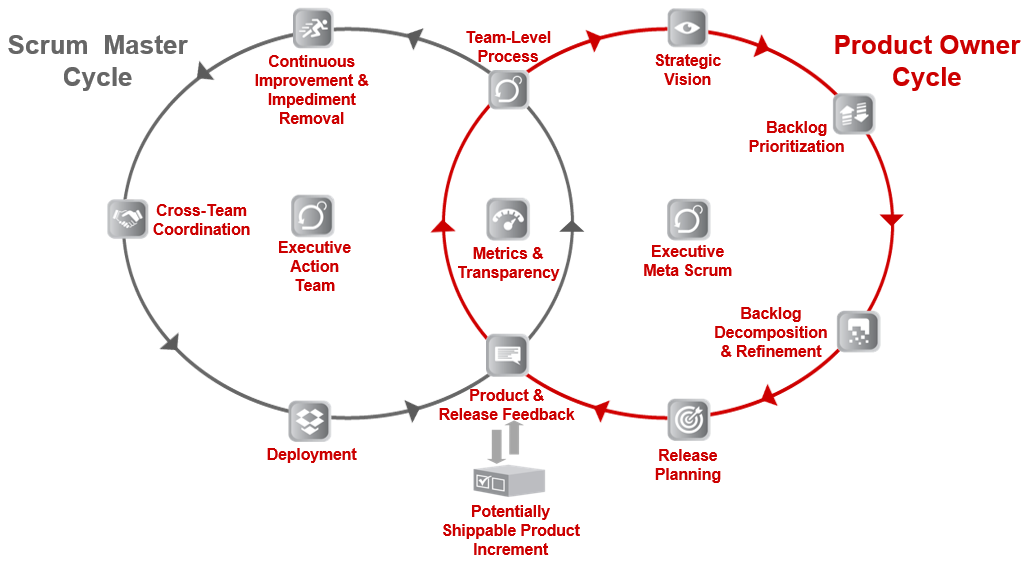
\includegraphics[width=1.0\linewidth]{SMPO-Cycle.png}

\subsection{Cultura guidata dai valori}

Oltre a separare la responsabilità del ``cosa'' e del ``come'' Scrum@Scale si propone inoltre di creare organizzazioni sane creando una cultura basata sui valori in un contesto empirico. I valori di Scrum sono: apertura, coraggio, focus, rispetto e impegno. Questi valori guidano un processo decisionale empirico, che dipende dai tre pilastri di trasparenza, ispezione e adattamento.

L'apertura supporta la trasparenza in tutto il lavoro ed i processi, senza la quale non c'è possibilità di ispezionarli onestamente e tentare di adattarli per il meglio. Il coraggio si riferisce alla capacità di prendere le decisioni difficili richieste per fornire valore il più rapidamente possibile ed in maniera innovativa.

Focus e impegno si riferiscono al modo con cui gestiamo i nostri obblighi lavorativi, mettendo come più alta priorità la consegna di valore al cliente. Infine, tutto questo deve avvenire in un ambiente basato sul rispetto per gli individui che svolgono il lavoro, senza il quale nulla può essere creato.

Scrum@Scale aiuta le organizzazioni a prosperare supportando un modello di leadership trasformazionale che promuova un ambiente lavorativo positivo con un ritmo sostenibile e mettendo l'impegno a consegnare valore visibile al cliente come frutto dei nostri sforzi.

\subsection{Come iniziare con Scrum@Scale}
Quando si intende implementare una grande rete di team, è fondamentale sviluppare prima un \textbf{Modello di Riferimento} con un piccolo gruppo di team. Qualsiasi carenza si implementi inizialmente, questa verrà poi amplificata quando si estende il metodo a molteplici team. Molti dei problemi iniziali di estensione del metodo saranno di tipo organizzativi, delle procedure e pratiche di sviluppo che bloccano i team dal raggiungere prestazioni elevate e creano frustrazione.

Pertanto, la prima sfida è creare un piccolo gruppo di team che implementino bene lo Scrum. Questo può essere fatto efficacemente creando un \textbf{Executive Action Team (EAT)}, responsabile della definizione ed implementazione della strategia di trasformazione. L'EAT deve essere composto da individui con la necessaria autorità, sia politica che finanziaria, per assicurarsi dell'esistenza del modello di riferimento. Questo insieme di team permette di risolvere gli impedimenti organizzativi che bloccano l'agilità e creare il modello di riferimento di Scrum che funzioni in quel contesto e che possa essere utilizzato come riferimento per l'estensione di Scrum in tutta l'organizzazione.

Via via che il modello di riferimento dei team si estende, gli ostacoli ed i colli di bottiglia che ritardano le consegne, producono sprechi o ostacolano l'agilità del business,  diventano visibili. Il modo più efficace per eliminare questi problemi è diffondere Scrum su tutta l'organizzazione in modo che l'intero flusso del valore sia ottimizzato.

Scrum@Scale permette di far scalare linearmente la produttività saturando l'organizzazione con Scrum e distribuendo il carico di lavoro e le responsabilità sulla qualità organicamente, in maniera consistente con la strategia, i prodotti ed i servizi dell'organizzazione stessa.

\section{Il ciclo degli Scrum Master}
\subsection{Processo a livello di Team}
Il \textbf{Processo a Livello di Team} costituisce il primo punto di contatto tra lo Scrum Master ed il ciclo dei Product Owner, ed è definito chiaramente nella Scrum Guide. È composto da tre artefatti, cinque eventi e tre ruoli. L'obbiettivo del processo a livello di Team è di:
\begin{itemize}
\item massimizzare il flusso di lavoro completato e verificato qualitativamente.
\item incrementare le performance del team nel corso del tempo.
\item operare in una maniera che sia sostenibile e di arricchimento per il Team.
\item accelerare il loop di feedback del cliente
\end{itemize}

\subsection{Coordinare il ``Come'' - Lo Scrum of Scrums}
Un insieme di Team che necessitino di coordinamento per poter consegnare valore al cliente, costituiscono uno \textbf{``Scrum of Scrums'' (SoS)}.

Questo è a sua volta un Team Scrum ed è responsabile, per ogni Sprint, della piena integrazione dell'insieme degli incrementi potenzialmente consegnabile di prodotto da tutti i team partecipanti. Uno SoS espleta le funzioni di un Release Team e deve essere in grado di consegnare direttamente valore al cliente. Per far questo efficacemente necessita di essere consistente con la Scrum Guide, che ha i propri ruoli, artefatti ed eventi:

Ruoli:

È necessario che lo SoS disponga delle competenze necessarie per consegnare un incremento di prodotto potenzialmente consegnabile completamente integrato al termine di ogni Sprint. (Potranno essere necessari degli esperti Architetti, responsabili Qualità ed altre competenze operative). Occorrerà una rappresentanza dei Product Owner per risolvere problematiche di priorità. Lo Scrum Master dello Scrum of Scrums è chiamato \textbf{Scrum of Scrums Master (SoSM)}.

Eventi:

Lo SoSM facilita l'evento di Backlog Refinement durante il quale gli impedimenti sono definiti ``pronti'' per essere rimossi, in che modo rimuoverli e come il team possa sapere che sono ``fatti''. Particolare attenzione dovrebbe essere posta alla Retrospettiva dello SoS in cui le rappresentanze dei Team condividano cosa hanno appreso ed i miglioramenti ai processi svolti dai vari team, in modo da uniformare queste pratiche nei vari Team sottostanti lo SoS.
Lo SoS ha la versione \textbf{Scalata del Daily Scrum (SDS)}. L'evento SDS riflette il Daily Scrum in modo da ottimizzare la collaborazione e le performance della rete di Team. Dato che lo SoS ha bisogno di rispondere in tempo reale agli impedimenti sollevati dai Team partecipanti, gli Scrum Master dei Team devono essere presenti alla versione Scalata del Daily Scrum. Occorrerà anche avere una rappresentanza dei Product Owner per risolvere eventuali problemi di priorità. Potrà poi partecipare qualsiasi persona tra i componenti dei Team, a seconda delle necessità.

Inoltre, l'evento SDS:

\begin{itemize}
\item ha una time-box di 15 minuti o meno.
\item deve parteciparvi una rappresentanza di ogni team, includendo il team dei Product Owner.
\item è un forum in cui i rappresentanti dei team discutono su cosa stia andando bene, cosa viene fatto e su come i team possano lavorare insieme in modo più efficace. Alcuni esempi di ciò che potrebbe essere discusso sono:
\begin{itemize}
\item Quali impedimenti incontra il mio Team che potrebbero ostacolare il raggiungimento dello Sprint Goal (o impattare la prossima release)? 
\item Sta, il mio Team, facendo qualcosa che possa impedire ad un altro Team di raggiungere il loro Sprint Goal (o impattare la prossima release)?
\item Abbiamo scoperto nuove dipendenze tra Team o abbiamo scoperto modi che possano risolvere le dipendenze esistenti?
\item Quali miglioramenti abbiamo scoperto che possono essere estesi agli altri team?
\end{itemize}
\end{itemize}

\subsection{Lo Scrum of Scrums Master(SoSM)}
Lo Scrum of Scrums Master (SoSM) è responsabile dei rilasci unificato del lavoro dei Team e deve:
\begin{itemize}
\item rendere il progresso del lavoro visibile.
\item creare un backlog degli impedimenti visibile all'organizzazione.
\item rimuovere gli impedimenti che i Team non riescono a risolvere da soli. 
\item facilitare la prioritizzazione degli impedimenti, con particolare attenzione alle dipendenze cross-team e la distribuzione del backlog. 
\item migliorare l'efficacia dello Scrum of Scrums.
\item lavorare fianco a fianco con i Product Owner per rilasciare un incremento di prodotto potenzialmente consegnabile alla fine di ogni Sprint.
\item coordinare il rilascio dei team secondo i piani di rilascio dei Product Owner.
\end{itemize}

\subsection{Scalare lo SoS}
Secondo la dimensione dell'organizzazione o implementazione, potrebbero essere necessari più di uno SoS per poter creare un prodotto molto complesso. In questi casi può essere creato uno \textbf{Scrum of Scrum of Scrums (SoSoS)} unendo più Scrum of Scrums. Il SoSoS è un modello organico di team Scrum che è infinitamente scalabile. Ogni SoSoS dovrebbe avere lo Scrum Master dello SoSoS e versioni scalate di ogni artefatto ed evento.

Scalando lo SoS si riduce il numero di canali di comunicazione all'interno dell'organizzazione in modo da incapsulare la complessità. Lo SoSoS si interfaccia con uno SoS nella stessa esatta maniera con cui uno SoS si interfaccia con un singolo Team Scrum, e questo permette una scalabilità lineare.

\pagebreak
Diagrammi di esempio:

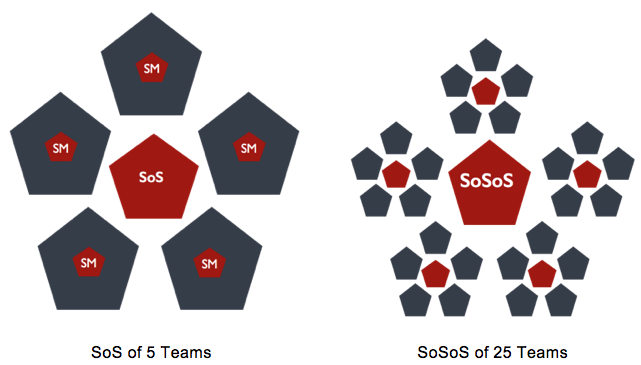
\includegraphics[width=1.0\linewidth]{Sos-R2.png}

\textbf{\textsc{nota:}} Anche se la Guida Scrum definisce la dimensione ottimale del Team da 3 a 9 persone, ricerche di Harvard hanno determinato che la dimensione ottimale di una  squadra è di 4,6 persone\footnote{Hackman, J Richard, Leading teams: Setting the stage for
great performances, Harvard Business Press, 2002}. Esperimenti con Team altamente performanti hanno ripetutamente dimostrato che 4 o 5 persone coinvolte nel lavoro è la dimensione ottimale. È essenziale per la scalabilità lineare che questo modello sia lo stesso anche per il numero di Team in un SoS. Pertanto, nella figura sopra e nei diagrammi seguenti, sono stati scelti dei pentagoni per rappresentare una squadra di 5 persone. Questi diagrammi sono pensati per essere solo di esempio, i diagrammi reali di una organizzazione possono essere anche molto diversi.

\subsection{Lo Executive Action Team}
Lo Scrum of Scrums di una intera organizzazione è chiamato \textbf{Executive Action Team (EAT)}. 

Il leadership team crea una bolla agile nell'organizzazione in cui il modello di riferimento opera con delle linee guida e procedure proprie in modo da integrarsi efficacemente con qualsiasi parte dell'organizzazione che non è ancora agile. È responsabile dell'ecosistema agile, implementa i valori di Scrum e si assicura che i ruoli Scrum siano creati e supportati.

L' EAT è il punto di arrivo per gli impedimenti che non possono essere risolti dagli SoS che li sollevano. Pertanto deve essere composto dagli individui che hanno potere politico e finanziario per rimuoverli. La funzione di un EAT è di coordinare molteplici SoS (o SoSoS) e di interfacciare le componenti non agilizzate dell'organizzazione. Esattamente come in ogni Team Scrum, l'EAT necessita di un PO e di uno SM. L'ottimo sarebbe se l'EAT si incontrasse giornalmente come ogni Scrum Team. Comunque devono incontrarsi almeno una volta a Sprint ed avere un backlog visibile.

%\pagebreak
Nel diagramma di esempio si mostra un EAT che coordina 5 gruppi di 25 team::

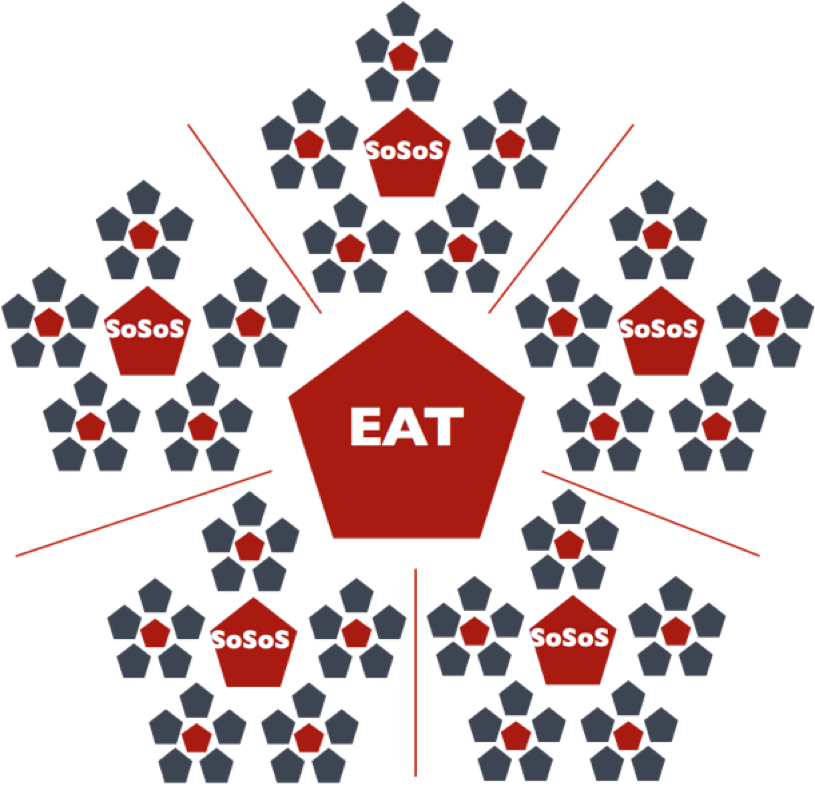
\includegraphics[width=\textwidth,height=\textheight,keepaspectratio]{SoS-EAT.png}

\subsection{Responsabilità e Backlog dell'EAT}
Scrum è un sistema operativo agile che differisce dal project management tradizionale.
L'intera organizzazione degli SM risponde all'EAT, che è responsabile di implementare questo sistema operativo agile stabilendo, mantenendo e migliorando la sua implementazione nell'organizzazione. Il ruolo dell'EAT è di creare un Backlog di Trasformazione Organizzativa (una lista ordinata di iniziative agile che necessitano di essere compiute) e di verificare che vengano compiute.

Per esempio, se c'è un sistema di sviluppo prodotto tradizionale nella vecchia organizzazione, occorrerà creare, implementare e supportare un nuovo sistema di sviluppo prodotto Agile. Questo supporterà tipicamente criteri di qualità e problemi di normativa meglio del vecchio metodo implementando in maniera differente le varie regole e linee guida. L'EAT si assicura che una organizzazione di Product Owner sia creata e finanziata e che questa sia rappresentata all'interno dell'EAT stesso in modo da supportare questi sforzi.

L'EAT è responsabile per la qualità dello Scrum all'interno dell'organizzazione.
Le sue responsabilità includono, anche se non si limitano solo a questo:
\begin{itemize}
\item creare un sistema operativo agile per il Modello di Riferimento che scali attraverso l'organizzazione, includendo le regole operative aziendali, le procedure e le linee guida che abilitino l'agilità.
\item misura e miglioramento della qualità dello Scrum nell'organizzazione.
\item costruzione delle capacità necessarie dell'organizzazione per una agilità di business 
\item creazione di un centro per l'apprendimento continuo per le professionalità Scrum.
\item supporto all'esplorazione di nuovi modi di lavorare.
\end{itemize}
Infine, l'EAT deve organizzare e supportare un'organizzazione di Product Owner attraverso un'associazione di PO che replichino la struttura dello SoS e scalino le funzioni di PO. Questi team di PO e stakeholder chiave sono noti come  \textbf{MetaScrums}.

\subsection{Azioni/Risultati del Ciclo degli Scrum Master}
L'organizzazione degli SM (SoS, SoSoS e EAT) lavora con un insieme per completare gli altri componenti del Ciclo degli Scrum Master: \textbf{Miglioramento Continuo e
 Rimozione Impedimenti, Coordinamento Cross-Team e Deployment (rilasci - ndt)}.

Gli obbiettivi del Miglioramento Continuo e Rimozione Impedimenti sono:
\begin{itemize}
\item identificare gli impedimenti ed inquadrarli come opportunità.
\item mantenere un ambiente sano e strutturato di prioritizzazione e rimozione degli impedimenti, e quindi verifica dei risultati dei miglioramenti.
\item assicurare la visibilità nell'organizzazione degli effetti dei cambiamenti.
\end{itemize}

Gli obiettivi del Coordinamento Cross-Team sono:
\begin{itemize}
\item coordinamento di processi simili attraverso diversi team collegati.
\item mitigare le dipendenze tra team in modo da assicurarsi che non diventino impedimenti.
\item mantenere allineate le regole e le guide linea dei team per un risultato consistente.
\end{itemize}

Dato che l'obbiettivo dello SoS è di funzionare come un release team (team responsabile dei rilasci - ndt), il Deployment del prodotto ricade nelle sue responsabilità, mentre ciò che è contenuto in ogni rilascio ricade nelle responsabilità dei Product Owner. Per cui, gli obiettivi del Deployment sono:
\begin{itemize}
\item consegnare un flusso consistente di prodotto finito ai clienti.
\item integrare il lavoro di diversi team in un unico prodotto ben integrato.
\item assicurare una esperienza cliente di alta qualità.
\end{itemize}

\section{Ciclo dei Product Owner}
\subsection{Coordinare il ``Cosa'' - Il MetaScrum}
Un gruppo di Product Owner che necessitino di coordinare un singolo backlog che alimenta una rete di Team sono chiamati un \textbf{MetaScrum}. Per ogni SoS c'è un MetaScrum associato. Un MetaScrum allinea le priorità dei Team lungo un singolo percorso in modo che questi possano coordinare i propri backlog e creare un buon allineamento con gli stakeholder in modo da supportare il backlog stesso. I Product Owner dei team sono responsabili della composizione e prioritizzazione del Backlog del proprio Team e possono attingere dal Backlog condiviso del MetaScrum o generare un backlog indipendente a loro descrizione.

A team's product owner is accountable for the composition and prioritization of the team backlog and may pull backlog from the shared metascrum backlog into the team backlog or generate independent backlog at his or her discretion.

I MetaScrum tengono una versione scalata del Backlog Refinement, il \textbf{Backlog Refinement Scalato} 
\begin{itemize}
\item Ogni PO di ogni team (o un suo rappresentante) deve partecipare.
\item Questo evento è un forum per i leader dell'azienda, gli stakeholder, o altri clienti per esprimere le loro preferenze.
\end{itemize}
Questo evento avviene con la frequenza necessaria per assicurarsi che il backlog sia "pronto", in ogni modo almeno una volta ogni Sprint.

Le funzioni principali del MetaScrum sono:
\begin{itemize}
\item creare una visione generale del prodotto e renderla visibile all'organizzazione.
\item costruire un buon allineamento con gli stakeholder chiave in modo da assicurarsi il supporto per l'implementazione del backlog.
\item generare un singolo backlog prioritizzato, assicurandosi di evitare duplicazioni del lavoro.
\item creare una minima ``Definition of Done'' (la definizione di fatto - ndr) che si applichi a tutti i team nello SoS.
\item eliminare e dipendenze evidenziate all'interno dello SoS stesso.
\item creare e coordinare un Piano dei Rilasci.
\item decidere e monitorare le metriche che forniscano delle indicazioni sul prodotto.
\end{itemize}
I MetaScrum, esattamente come i SoS, lavorano a loro volta come dei Team Scrum. Pertanto necessitano di qualcuno che funzioni da SM e mantenga il Team in pista nelle discussioni. Essi necessitano inoltre di una singola persona che è responsabile di coordinare la generazione di un singolo Product Backlog per tutti i team che il MetaScrum rappresenta. Questa persona è designata per essere lo \textbf{Chief Product Owner} (Product Owner Capo - ndt).

\subsection{Lo Chief Product Owner (CPO)}
Grazie ai MetaScrum, gli Chief Product Owner coordinano le priorità tra i Product Owner che sono impegnati con i singoli team. Essi allineano le priorità nel backlog secondo i bisogni degli Stakeholder e clienti. Esattamente come nel caso dello SoSM (Lo Scrum Master dello Scrum of Scrum - ndt), essi possono essere uno dei PO che decida di impersonare anche questo ruolo, oppure una persona specificatamente dedicata. Le loro responsabilità sono le stesse dei normali PO, ma ad una scala diversa: 
\begin{itemize}
\item Impostano una visione strategica dell'intero prodotto.
\item Creano un singolo backlog prioritizzato di valore per essere lavorato da tutti i team.
\begin{itemize}
\item Questi elementi di Backlog potranno essere più grandi di quelli su cui lavora un PO di un singolo team.
\end{itemize}
\item Lavorando fianco a fianco con lo Scrum Master dello SoS associato in modo che il piano di rilascio generato dal MetaScrum possa essere consegnato efficientemente.
\item Monitorare il feedback dei clienti sul prodotto in modo da adattare il backlog di conseguenza.
\end{itemize}

\subsection{Scalare il MetaScrum}
Così come gli SoS possono crescere in SoSoS, anche i MetaScrum possono espandersi con lo stesso meccanismo. Non c'è un termine associato specifico per queste unità espanse, e non si fornisce un titolo esteso per i CPO. Si incoraggia ogni organizzazione a sviluppare i propri titoli. Nei diagrammi seguenti è stato scelto di aggiungere dei ``Chief'' aggiuntivi di fronte al titolo PO via via che salgono di grado.

%\pagebreak
Alcuni diagrammi di esempio:

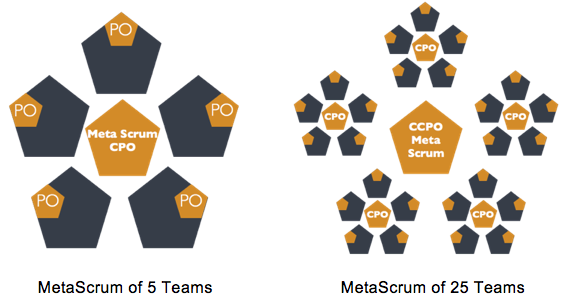
\includegraphics[width=1.0\linewidth]{MetaScrum-R2.png}

\textbf{NOTA:} Come già menzionato, i pentagoni rappresentano la dimensione ideale dei Team Scrum dei MetaScrum. Questi diagrammi sono pensati per essere solo di esempio, le organizzazioni reali possono differire di molto.

\subsection{Lo Executive MetaScrum (EMS)}
Il MetaScrum abilita il disegno di una rete di Product Owner che scala infinitamente di fianco agli SoS associati. Il MetaScrum di una organizzazione intera è chiamato \textbf{Executive MetaScrum}. Lo EMS delinea la visione dell'intera organizzazione ed imposta le priorità strategiche per l'intera azienda, allineando tutti i team attorno un obiettivo comune.

Diagramma di esempio di un EMS che coordina 5 gruppi di 25 team:

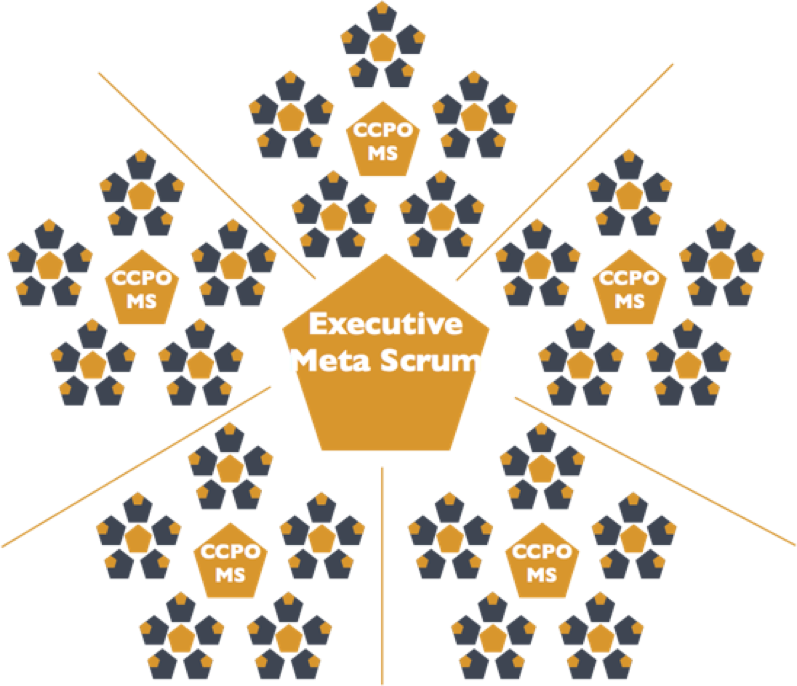
\includegraphics[width=1.0\linewidth]{ExecMetaScrum.png}

\subsection{Azioni e risultati dell'Organizzazione dei Product Owner}
L'organizzazione dei PO (i vari MetaScrum, lo CPO e l'Executive MetaScrum) lavorano con un tutt'uno per soddisfare i componenti del ciclo dei Product Owner: \textbf{Visione Strategica, Prioritizzazione del Backlog, Decomposizione del Backlog e Raffinamento, Piano dei Rilasci}.

Gli obiettivi dell'impostare una "Visione Strategica" sono:
\begin{itemize}
\item allineare chiaramente l'organizzazione intera attorno un percorso condiviso.
\item articolare in modo convincente il motivo per cui l'organizzazione esiste.
\item descrivere cosa farà l'organizzazione per sfruttare le risorse chiave a supporto della sua missione.
\item rispondere rapidamente alle mutevoli condizioni del mercato.
\end{itemize}
Gli obiettivi della "Prioritizzazione del Backlog" sono:
\begin{itemize}
\item identificare un ordinamento chiaro dei prodotti, funzionalità e servizi che dovranno essere consegnati.
\item riflettere nell'ordinamento del backlog la creazione del valore, la mitigazione dei rischi e delle dipendenze interne.
\item prioritizzare un'iniziativa ad alto livello attraverso l'intera organizzazione agile prima della "Decomposizione del Backlog e Raffinamento"
\end{itemize}
Gli obiettivi della "Decomposizione del Backlog e Raffinamento" sono di:
\begin{itemize}
\item scomporre prodotti e progetti complessi in elementi funzionali indipendenti che possano essere completati da un singolo team in uno Sprint.
\item catturare e distillare i requisiti emergenti e i feedback dei clienti.
\item assicurarsi che gli elementi del backlog siano veramente ``Pronti'' in modo che possano essere presi dai singoli team.
\end{itemize}
Gli obiettivi del "Piano dei Rilasci" sono di:
\begin{itemize}
\item mettere a piano il rilascio delle funzionalità e caratteristiche chiave.
\item comunicare le aspettative di consegna agli stakeholder.
\item aggiornare la prioritizzazione, quando necessario.
\end{itemize}

\section{Connessione dei cicli del PO e degli SM}

\subsection{Comprensione del Feedback}
Il componente \textbf{Feedback} è il secondo punto in cui i cicli dei PO e degli SM 
si toccano. Il Feedback sul prodotto guida il miglioramento continuo attraverso l'adattamento del Product Backlog mentre il Feedback sul rilascio guida i miglioramenti continui attraverso i meccanismi di Deployment. Gli obiettivi di ottenere e analizzare il Feedback sono di:
\begin{itemize}
\item validare le nostre assunzioni.
\item comprendere come i clienti usano ed interagiscono con il prodotto.
\item trovare idee per nuove caratteristiche e funzionalità.
\item definire miglioramenti alle funzionalità esistenti.
\item aggiornare il progresso rispetto il completamento del prodotto/progetto in modo
da aggiornare il piano dei rilasci e allineare le le aspettative degli stakeholder.
\item identificare i miglioramenti dei metodi e meccanismi di deployment.
\end{itemize}

\subsection{Metriche e Trasparenza}
Una radicale trasparenza è essenziale per far funzionale lo Scrum in maniera ottimale,
e questo è possibile solo se l'organizzazione abbraccia i valori dello Scrum.
Questo fornisce all'azienda la capacita di valutare il proprio progresso onestamente
e di ispezionare ed adattare i propri prodotti e processi. Questi sono le fondamenta
della natura empirica di Scrum, come descritto nella Scrum Guide.

Entrambi i cicli degli SM e dei PO richiedono delle metriche decise separatamente
dall'organizzazione degli SM e dei PO. Le metriche potranno essere uniche sia per
organizzazioni specifiche che per specifiche funzioni all'interno dell'organizzazione.
Scrum@Scale non richiede un insieme specifico di metriche ma ne suggerisce un
minimo. L'organizzazione dovrebbe misurare:
\begin{itemize}
\item Produttività - ad esempio cambiamenti nelle quantità di prodotto funzionante
consegnato per ogni Sprint.
\item Valore consegnato - ad esempio Valore di Business per ogni unità di produttività del Team.
\item Qualità - ad esempio il tasso di difettosità o indisponibilità del servizio.
\item Sostenibilità - ad esempio il morale del team.
\end{itemize}
L'obiettivo di avere "Metriche e Trasparenza" è di:
\begin{itemize}
 \item fornire a tutti coloro che devono prendere decisioni, compresi i membri dei
 team, una comprensione appropriata del contesto in modo da permettere delle
 buone decisioni.
\item accorciare il ciclo di feedback il più possibile in modo da evitare correzioni eccessive.
\item ridurre gli sforzi aggiuntivi per i team, stakeholder ed i leader dell'azienda.
 \end{itemize}

\subsection{Alcune note sul Disegno dell'Organizzazione}
L'architettura scale-free (ad invarianza di scala - ndt) permette di disegnare organizzazioni
basate su componenti, proprio come è costituito il framework stesso. Questo permette di
ribilanciare o rifattorizzare i Team in risposta ai bisogno del mercato. Durante la crescita
di una organizzazione, comprendere i benefici di avere team distribuiti può essere importante. Alcune organizzazioni raggiungono talenti altrimenti non disponibili e sono
in grado di espandersi e contrattualizzare dello sviluppo in outsourcing secondo il bisogno. Scrum@Scale mostra in che modo fare questo evitando ritardi dei tempi,
compromissione della comunicazione, qualità inferiore ed abilitando una scalabilità
lineare sia in dimensione che nella distribuzione geografica. \footnote{Sutherland, Jeff and Schoonheim, Guido and Rustenburg, Eelco and Rijk, Maurits, ``Fully distributed scrum:
The secret sauce for hyperproductive offshored development teams'',
AGILE'08. Conference, IEEE: 339-344, 2008}

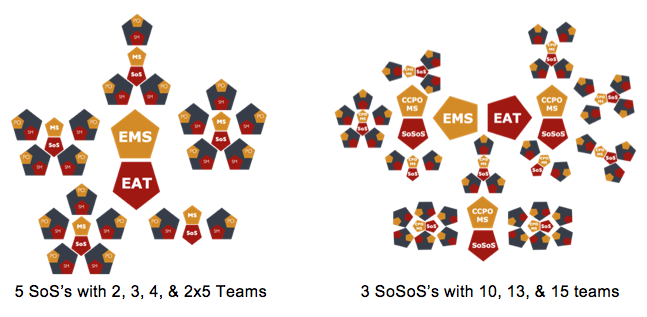
\includegraphics[width=1.0\linewidth]{VariableSoS-R2.png}
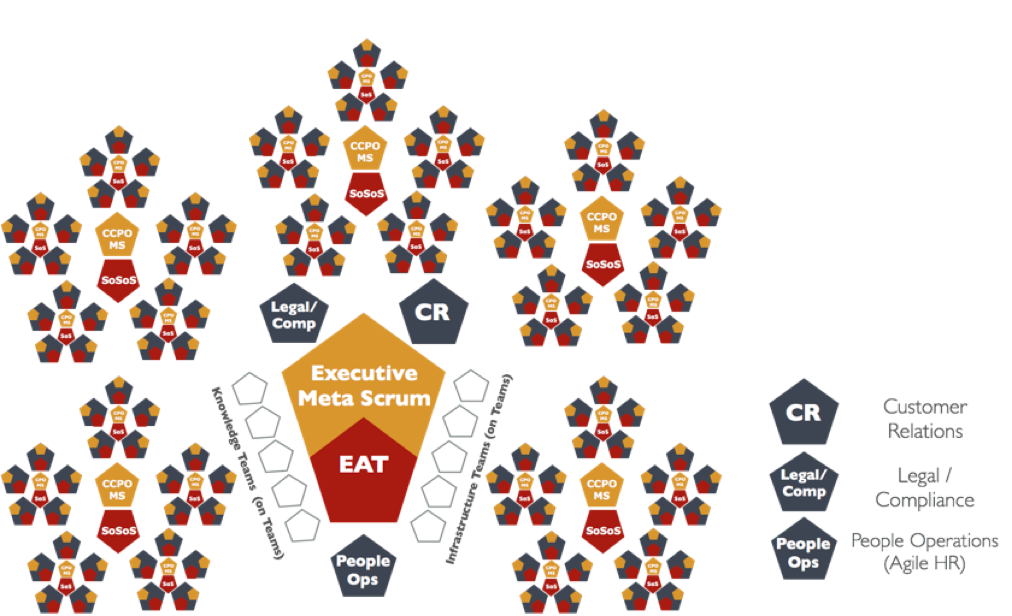
\includegraphics[width=1.0\linewidth]{OrganizationalDiagram.png}

In quest'ultimo diagramma organizzativo i \textbf{Knowledge Team e gli Infrastructure
Team} rappresentano dei team virtuali di specialisti, numericamente troppo pochi per essere allocati in ogni team. Questi si coordinano come un Team Scrum, tenuti assieme tramite dei livelli di servizio (conosciuti anche come SLA, service-level agreement - ndt) ove le richieste fluiscono attraverso un PO per ogni specialità che le converte in un backlog ordinato e trasparente. Molto importante è da notare che questi team NON sono dei silos di individui che siedono assieme (motivo per cui sono rappresentati come pentagoni vuoti); i membri di questi Team siedono nei Team Scrum con cui lavorano, ma sono parte individualmente di  questo Team Scrum Virtuale per gestire il backlog disseminato (specifico della competenza - ndt) ed il miglioramento dei propri processi.

\textbf{I responsabili delle Relazioni con la Clientela, i responsabili Legali e Compliance ed i responsabili del Personale (Agile HR)} sono inclusi in questo diagramma in quanto sono parte necessaria dell'organizzazione ed esisteranno come team Scrum Indipendenti, da cui dipendono tutti gli altri Team Scrum.

Nota finale riguardo la rappresentazione dell'EAT e dello EMS: in questo diagramma sono mostrati come sovrapposti in quanto alcuni membri siedono in entrambe le organizzazioni. In organizzazioni o implementazioni molto piccole, l'EAT e lo EMS possono interamente consistere nelle stesse persone.

\section{Note Finali}
Scrum@Scale è disegnato per scalare la produttività ed avere l'intera organizzazione produrre il doppio del lavoro in metà tempo mantenendo alta qualità ed un significativo miglioramento dell'ambiente lavorativo. Le grandi organizzazioni che implementino appropriatamente il framework potranno ridurre i costi dei loro prodotti e servizi migliorando la qualità e l'innovazione.

Scrum@Scale è disegnato per saturare una organizzazione con Scrum. Tutti i Team,
incluso i Leader, le Risorse Umane, i Legali, la Consulenza, il Training ed i team dei Prodotti e Servizi implementano lo stesso stile di Scrum razionalizzando e migliorando l'organizzazione stessa.

Uno Scrum ben implementato può far funzionare un'intera organizzazione.

\section{Riconoscimenti}
Si riconosce a IDX la creazione dello Scrum of Scrum che per primo ha permesso di scalare Scrum a centinaia di Team,\footnote{Sutherland, Jeff,
``Inventing and Reinventing SCRUM in five Companies'', Sur le site officiel
de l'alliance agile, 2001} PatientKeeper per la creazione del MetaScrum,\footnote{Sutherland, Jeff, ``Future of scrum: Parallel pipelining
of sprints in complex projects'', Proceedings of the Agile Development
Conference,  IEEE Computer Society 90-102,  2005.}  che ha permesso lo sviluppo rapido ed innovativo del prodotto ed OpenView Venture Partners per aver esteso Scrum all'intera organizzazione.\footnote{Sutherland, Jeff and Altman,
Igor, ``Take no prisoners: How a venture capital group does scrum'', Agile
Conference, 2009. AGILE'09, IEEE 350-355.  2009} Diamo inoltre credito ai suggerimenti di Intel che, con oltre 25.000 persone che lavorano con Scrum, ci hanno insegnato che ``niente scala'' tranne l'architettura scale-free, e SAP che, con la più grande organizzazione prodotto Scrum, ci ha insegnato che il coinvolgimento del management nel MetaScrum è essenziale per far lavorare assieme 2.000 Team Scrum.

Gli Agile Coach e Trainer che hanno implementato questi concetti in Amazon, GE, 3M, Toyota, Spotify, Maersk, Comcast, AT\&T ed in molte alte aziende, lavorando con Jeff Sutherland sono stati di grande aiuto nel verificare questi concetti su un ampissimo raggio di aziende di differenti domini.

Ed infine Avi Schneier ed Alex Sutherland, inestimabili nella stesura e nella formattazione di questo documento.

\section{Note alla traduzione italiana}
Traduzione a cura di \textbf{Paolo Sammicheli}, Scrum@Scale Trainer. Nel corso della traduzione è stato scelto di mantenere inalterati i termini sprovvisti di una traduzione ovvia in modo da evitare incomprensioni ed impedire agli utenti di questa guida di trovare facilmente il corrispettivo termine nell'ampissima documentazione online in Inglese, presente e futura. Laddove occorreva una chiarificazione dei termini, questa è stata aggiunta tra parentesi con la sigla Nota del Traduttore (NDT).

\pagebreak

\printbibliography



\end{document}
